\documentclass[12pt,letterpaper]{article}

% text and symbol support
\usepackage[utf8]{inputenc}
\usepackage[T1]{fontenc}
\usepackage{textcomp}
\usepackage{amsmath, amssymb, amsthm}
\usepackage[normalem]{ulem}
\useunder{\uline}{\ul}{}

% formatting support
\usepackage{framed}
\usepackage[page]{appendix}
\usepackage{authblk}
\usepackage{fancyhdr}
\usepackage{lscape}

% figure support
\usepackage{import}
\usepackage{xifthen}
\pdfminorversion=7
\usepackage{pdfpages}
\usepackage{transparent}
\newcommand{\incfig}[1]{%
  \def\svgwidth{\columnwidth}
  \import{./figures/}{#1.pdf_tex}
}
\usepackage{pgfplots}
\pgfplotsset{width=7cm,compat=1.18}
\usepackage[section]{placeins}
\usepackage{subcaption}
\captionsetup{subrefformat=parens}
\usepackage{graphicx}

% table support
\usepackage{booktabs}
\usepackage{longtable}
\usepackage{array}

% bibliography support
\usepackage[backend=biber,style=apa]{biblatex}
\addbibresource{references.bib}

% additional packages
\usepackage{lipsum, verbatim, siunitx, tcolorbox}
\sisetup{detect-family}

% command definitions
\newcommand{\C}{\mathbb{C}}
\newcommand{\R}{\mathbb{R}}
\newcommand{\Q}{\mathbb{Q}} 
\newcommand{\D}{\mathbb{D}}
\newcommand{\Z}{\mathbb{Z}}
\newcommand{\N}{\mathbb{N}}

% other package settings
\pdfsuppresswarningpagegroup=1
\usepackage{lmodern}

\makeatletter
\newread\pin@file
\newcounter{pinlineno}
\newcommand\pin@accu{}
\newcommand\pin@ext{pintmp}
% inputs #3, selecting only lines #1 to #2 (inclusive)
\newcommand*\partialinput [3] {%
  \IfFileExists{#3}{%
    \openin\pin@file #3
    % skip lines 1 to #1 (exclusive)
    \setcounter{pinlineno}{1}
    \@whilenum\value{pinlineno}<#1 \do{%
      \read\pin@file to\pin@line
      \stepcounter{pinlineno}%
    }
    % prepare reading lines #1 to #2 inclusive
    \addtocounter{pinlineno}{-1}
    \let\pin@accu\empty
    \begingroup
    \endlinechar\newlinechar
    \@whilenum\value{pinlineno}<#2 \do{%
      % use safe catcodes provided by e-TeX's \readline
      \readline\pin@file to\pin@line
      \edef\pin@accu{\pin@accu\pin@line}%
      \stepcounter{pinlineno}%
    }
    \closein\pin@file
    \expandafter\endgroup
    \scantokens\expandafter{\pin@accu}%
  }{%
    \errmessage{File `#3' doesn't exist!}%
  }%
}
\makeatother

\usepackage{geometry}
\usepackage{pdflscape}
\usepackage{threeparttable}    
\usepackage{dcolumn}    % aligning decimals
    \newcolumntype{d}[1]{D{.}{.}{#1}}

\usepackage{draftwatermark}
\SetWatermarkText{\textsc{draft}}
\SetWatermarkScale{1.5}
\SetWatermarkColor[gray]{0.95}

\usepackage[bottom]{footmisc}

% Title
\title{Reopening After Covid: A Replication of \citeauthor{Chetty2020}'s ``The Economic Impacts of COVID-19.''}

% My name
\author[1]{Annais Gangolf\thanks{agangolf@haverford.edu}}
\author[1]{Devansh Goyal\thanks{dgoyal@haverford.edu}}
\author[1]{Samuel E. Ross\thanks{seross@haverford.edu}}
  \affil[1]{Economics Research Club, Haverford College, Haverford, PA 19041, USA}
\date{\today}
\setcounter{Maxaffil}{0}
\renewcommand\Affilfont{\itshape\small}

\begin{document}

\maketitle

\abstract{During the Covid pandemic, many policies were implemented without knowledge of their economic impacts. In this paper, we investigate the efficacy of one policy---state-ordered reopenings---by replicating a portion of \textcite{Chetty2020}, who assemble a high-frequency database containing measures of economic health using anonymized data from private companies. They use an event study approach to compare the economic trajectory of the first several states to reopen with a set of controls, finding that the policy had only modest positive effects on spending, employment, business activity, and mobility. These results are broadly consistent with a growing literature on pandemic mandates’ economic impacts. We obtain qualitatively similar estimates to \citeauthor{Chetty2020} although we fail to precisely replicate their results, finding discrepancies in magnitude, direction, and sample size. Despite these differences, we agree with \citeauthor{Chetty2020}’s conclusion that mandates’ economic impacts were modest and that pandemic-driven changes in economic activity were more driven by consumers’ health concerns than policy restrictions, raising questions about stay-at-home orders’ use in future health crises.
}

\section*{Introduction}
The Covid pandemic was an unprecedented challenge for modern economic and political leaders. Rapid policy response was essential to aid recovery from the quick economic downturn. Reform was key as structural vulnerabilities were exposed. In many cases, though, guidelines were hastily implemented with their economic impacts unknown. As climate change and globalization make pandemics ever more likely, it is crucial that we learn from our reaction to the Covid crisis, studying the things that worked, and taking note of those that didn’t.

In this paper, we replicate a portion of \textcite{Chetty2020}, who provide a vital resource for research on the pandemic response by constructing a real-time database that tracks key measures of economic health. They use these data to analyze a wide range of legislation, including the 2020 stimulus payments, Paycheck Protection Program, and unemployment benefit increases. Our paper focuses on one of these measures: state-ordered reopenings and their heterogenous impact on consumer spending, employment, small business revenues, and how much time people spend away from home. 

\citeauthor{Chetty2020} find that state-ordered reopenings result in modest increases in spending, unemployment, and small businesses open, concluding that an economic recovery (or lack thereof) is more affected by consumers’ health concerns than government mandates. These findings are consistent with a growing literature concerning the economic impacts of pandemic mandates (\textcite{Bartik2020}, \textcite{Goolsbee2020}). \citeauthor{Bartik2020} use private employment data to find that layoffs largely took place before stay-at-home orders went into effect, policy only driving a small share of overall job losses. \citeauthor{Goolsbee2020} show that mobility declined well before lockdowns were enacted, their total effect being comparatively minor. They find that shutdowns also shifted consumer spending from nonessential to essential businesses, implying that mandate-driven changes in economic indicators may be heterogenous across industries. 

We replicate the methodology of \citeauthor{Chetty2020} to produce estimates of reopenings’ impacts on broad measures of economic health. Our model is an event study with a difference-in-differences identification approach. For data processing, we group the first five US states that reopened by their event date, identify control states with similar prior patterns in economic indicators, and define time relative to this reopening date, stacking the five states’ series. We then perform our regressions, limiting our window of analysis to the two weeks before and after reopening.

We find that state-ordered reopenings cause uniform increases in consumer spending, employment, small business activity, and mobility, being robust to changes in analysis window and data aggregation techniques. Our results are broadly consistent with those of \citeauthor{Chetty2020}, but we fail to precisely replicate their numerical estimates and graphs. We speculate that these discrepancies may have arisen from the anonymization process---missing values being prevalent in the public database---or our own misinterpretation of methodology sections that we found ambiguous. These differences aside, we maintain the conclusion that state-mandated reopenings had modest positive economic effects, with businesses’ and consumers’ health preferences likely driving the majority of indicator movement.

Our paper proceeds as follows. Section 2 summarizes the database developed by \citeauthor{Chetty2020} and describes the specific series used in our replication. Section 3 describes our methodology and data processing. Section 4 reports our findings and discusses numerical discrepancies with \citeauthor{Chetty2020}. Section 5 concludes.

\section*{Data}
\citeauthor{Chetty2020} construct a public database that tracks key economic indicators like consumer spending, small business revenues, employment rates, and GPS mobility at a postal-code level. All series in the dataset are available from January 2020 to the time of writing (i.e., October 2022). 

They create these series by aggregating data from several private companies. The consumer spending indicator uses internal data from Affinity Solutions, a company that “combines consumer credit and debit information to support financial service products, such as loyalty programs for credit card companies.” The employment rate data is aggregated from three companies: Paychex, Intuit, and Earnin. The former two facilitate payroll services for small and medium-sized businesses, while the latter is a financial management application that provides access to paychecks before deposit. They source small business data  from Womply, a company that provides analytical services to small businesses by aggregating data from credit card processors Finally, data on geographic mobility is drawn from Google’s Community Mobility Reports, recording the amount of time people spend away from home at public spaces like parks, schools, and grocery stores. In addition to the indicators that we use, the database contains other series such as job postings, unemployment benefit claims, and Covid cases.

The data were processed and anonymized to protect confidential consumer information, remove seasonality, and minimize large daily fluctuations. This included using a seven-day moving average and transforming indices to reflect percentage changes from their mean in 4--31 January 2020.  

To study the effects of state-level reopening orders, the concern of this replication, \citeauthor{Chetty2020} use their state-level data series on consumer spending, business revenues, employment rates, and geographical mobility. For all series except for employment rates, we use the publicly available data from the Opportunity Insights website. For employment, we identified missing values for Washington D.C. in the public data, so we contacted the paper’s authors for a more complete dataset, which we use.

\section*{Methods}
We replicate \citeauthor{Chetty2020} by using a difference-in-differences (DiD) event-study model to estimate the effect of reopening on consumer spending, employment, small businesses open, and time spent outside home. 

We begin by defining our treatment group as the first five states which reopened in any capacity: South Carolina on 20 April 2020, Alaska and Georgia on 24 April 2020, and Minnesota and Mississippi on 27 April 2020. Each of these dates is associated with four sets of control states which had similar trends in each respective economic indicator of concern before reopening (see \citeauthor{Chetty2020}, Appendix Table 6).

For each event-indicator group, we drop states which are neither treated nor controls and code dummy variables for (1) whether the observation is from a treated or control state, (2) whether the observation is from past the reopening date, and (3) their interaction. Next, we define time relative to the date of reopening (e.g., $t=0$ is 20 April 2020 in the first case) and stack the three events for each indicator. This allows us to regress the indicator against the three aforementioned dummy variables for a two week window about the event date, the estimated effect of reopening on the indicator being the coefficient on the interaction term. We also perform the same regression with a three week window for robustness.

\section*{Results}
We display our regression results in the second panel of Table~\ref{tab:reg1}. Using our DiD method, we estimate that reopening from a Covid lockdown results in increases of consumer spending by 0.33\%, employment by 1.02\%, small businesses open by 2.91\%, and time spent outside home by 0.73\%. These results are robust to expanding the regression window to three weeks, with all effects being identical in direction and greater in magnitude than the original estimates.

We plot the average value of the respective indicators for treatment and control states in Figures~\ref{fig:spend}, \ref{fig:emp}, and \ref{fig:merchants}. As is visible, treated and control states follow approximately parallel trends before reopening and moderately diverge after reopening, commensurate with our DiD estimates. However, there is a comparable divergence between the series before

The first panel of Table~\ref{tab:reg1} and Figures~\ref{fig:spendC}, \ref{fig:empC}, and \ref{fig:merchantsC} display the original results of \citeauthor{Chetty2020} in contrast with our own. While our regressions give qualitatively similar estimates to theirs, discrepancies exist in the precise magnitude of effects and in sample size. In some cases, these gaps are relatively small: with a two week analysis window, we estimate a 1.02\% increase in employment as an effect of reopening while \citeauthor{Chetty2020} estimate a 0.65\% increase---both using 208 observations. However, in the case of open small businesses with a two-week window, our estimate of a 2.91\% increase differs significantly from their estimate of a 0.30\% decrease. Further, our two and three week windows used 244 and 366 observations respectively, while both of theirs use 248. These unchanging sample sizes are especially puzzling. We lack a sound explanation for many of these discrepancies, but there were some uncertainties during the replication that may have contributed.

First, while data were supplied at a daily frequency, \citeauthor{Chetty2020} performed their analysis with weekly observations. Given that the data were provided as seven day moving averages, we constructed our weekly series by dropping all observations but Sundays; however, this operation was not directly specified by their paper. 

Their graphs in Figures~\ref{fig:spendC}, \ref{fig:empC}, and \ref{fig:merchantsC} bring up another issue: the stacked series all appear to be drawn from weekly data, the nearest point to the event being the day prior. For the opening dates 20 and 27 April 2020---both Mondays---, this corresponds to the data being Sunday-based, as we’d expect. However, their figures also imply that the series for the opening date 24 April 2020, a Thursday, is Wednesday-based. To reconcile this, we create our graphs using the Wednesday-based series for the 24 April date while we perform our regression analysis using the uniformly Sunday-based series. For robustness, we also ran our regressions using the alternative aggregating method, finding similar results.

Finally, there are several unclear specifications. \citeauthor{Chetty2020} fail to describe whether they coded each treated state as open on the reopening date itself and they lack a complete definition for the analysis window; that is, “the two weeks before the reopening in the treated states and two weeks after” could mean $-14 \le t \le 14$, $-13 \le t \le14$, or $-14 \le t \le -13$. Respectively, we code the reopening date as open and calculate the analysis window using the first variation, but our results are robust to all these choices.

\section*{Discussion}
[TBD]

\clearpage

\printbibliography

% TABLES
\begin{landscape}
    \begin{table}[b]\centering
      \def\sym#1{\ifmmode^{#1}\else\(^{#1}\)\fi}
      \caption{OLS Regression results for state-level reopenings. \label{tab:reg1}}
      \begin{tabular}{r*{9}{c}}
        \toprule
        & \multicolumn{2}{c}{Spending (\%)} & \multicolumn{2}{c}{Employment (\%)}& \multicolumn{2}{c}{Small Businesses}& \multicolumn{2}{c}{Time Outside}\\
        Dep. Var.:      &&&&& \multicolumn{2}{c}{Open (\%)} & \multicolumn{2}{c}{Home (\%)} \\
        \midrule
        \addlinespace
        \multicolumn{1}{l}{\textbf{Panel A: \textcite{Chetty2020}}}&\multicolumn{1}{c}{(1)}&\multicolumn{1}{c}{(2)}&\multicolumn{1}{c}{(3)}&\multicolumn{1}{c}{(4)}&\multicolumn{1}{c}{(5)}&\multicolumn{1}{c}{(6)}&\multicolumn{1}{c}{(7)}&\multicolumn{1}{c}{(8)}       \\
        \cmidrule(lr){2-3} \cmidrule(lr){4-5} \cmidrule(lr){6-7} \cmidrule(lr){8-9} 
        DiD Estimate of Effect  &  1.43 &  1.37 &  0.65 &  1.04 &  -0.30 &  1.26 & 3.27 &  4.44  \\
          & (0.51) & (0.53)& (0.51)& (0.97)& (0.85)& (0.88)& (1.26)& (1.85)    \\
        \addlinespace
        N  &  \multicolumn{1}{c}{200}&  \multicolumn{1}{c}{312}&  \multicolumn{1}{c}{208}&  \multicolumn{1}{c}{258}&  \multicolumn{1}{c}{248}&  \multicolumn{1}{c}{248}&  \multicolumn{1}{c}{244}&  \multicolumn{1}{c}{324}\\
        \addlinespace
        Analysis Window (Weeks)         &  \multicolumn{1}{c}{2}            & \multicolumn{1}{c}{3}&  \multicolumn{1}{c}{2}            & \multicolumn{1}{c}{3}&  \multicolumn{1}{c}{2}            & \multicolumn{1}{c}{3}&  \multicolumn{1}{c}{2}            & \multicolumn{1}{c}{3}             \\
        \addlinespace
        \midrule
        \addlinespace
      \multicolumn{1}{l}{\textbf{Panel B: Replication}}&\multicolumn{1}{c}{(1)}&\multicolumn{1}{c}{(2)}&\multicolumn{1}{c}{(3)}&\multicolumn{1}{c}{(4)}&\multicolumn{1}{c}{(5)}&\multicolumn{1}{c}{(6)}&\multicolumn{1}{c}{(7)}&\multicolumn{1}{c}{(8)}       \\
        \cmidrule(lr){2-3} \cmidrule(lr){4-5} \cmidrule(lr){6-7} \cmidrule(lr){8-9} 
        \partialinput{4}{5}{RegTab.tex}
        \addlinespace
        \partialinput{7}{7}{RegTab.tex}
        \addlinespace
        Analysis Window (Weeks)         &  \multicolumn{1}{c}{2}            & \multicolumn{1}{c}{3}&  \multicolumn{1}{c}{2}            & \multicolumn{1}{c}{3}&  \multicolumn{1}{c}{2}            & \multicolumn{1}{c}{3}&  \multicolumn{1}{c}{2}            & \multicolumn{1}{c}{3}             \\
        \addlinespace
        \bottomrule
        \multicolumn{8}{l}{\footnotesize Standard errors clustered by state in parentheses; significance levels not given in Chetty (2020).}\\
        \multicolumn{8}{l}{\footnotesize Data source: Opportunity Insights Economic Tracker.}\\
        \multicolumn{8}{l}{\footnotesize \sym{*} \(p<0.10\), \sym{**} \(p<0.05\), \sym{***} \(p<0.01\)}\\
      \end{tabular}
    \end{table}
\end{landscape}

% FIGURES
\begin{figure}
    \centering
    \caption{}
    \begin{subfigure}[t]{0.8\textwidth}
        \centering
        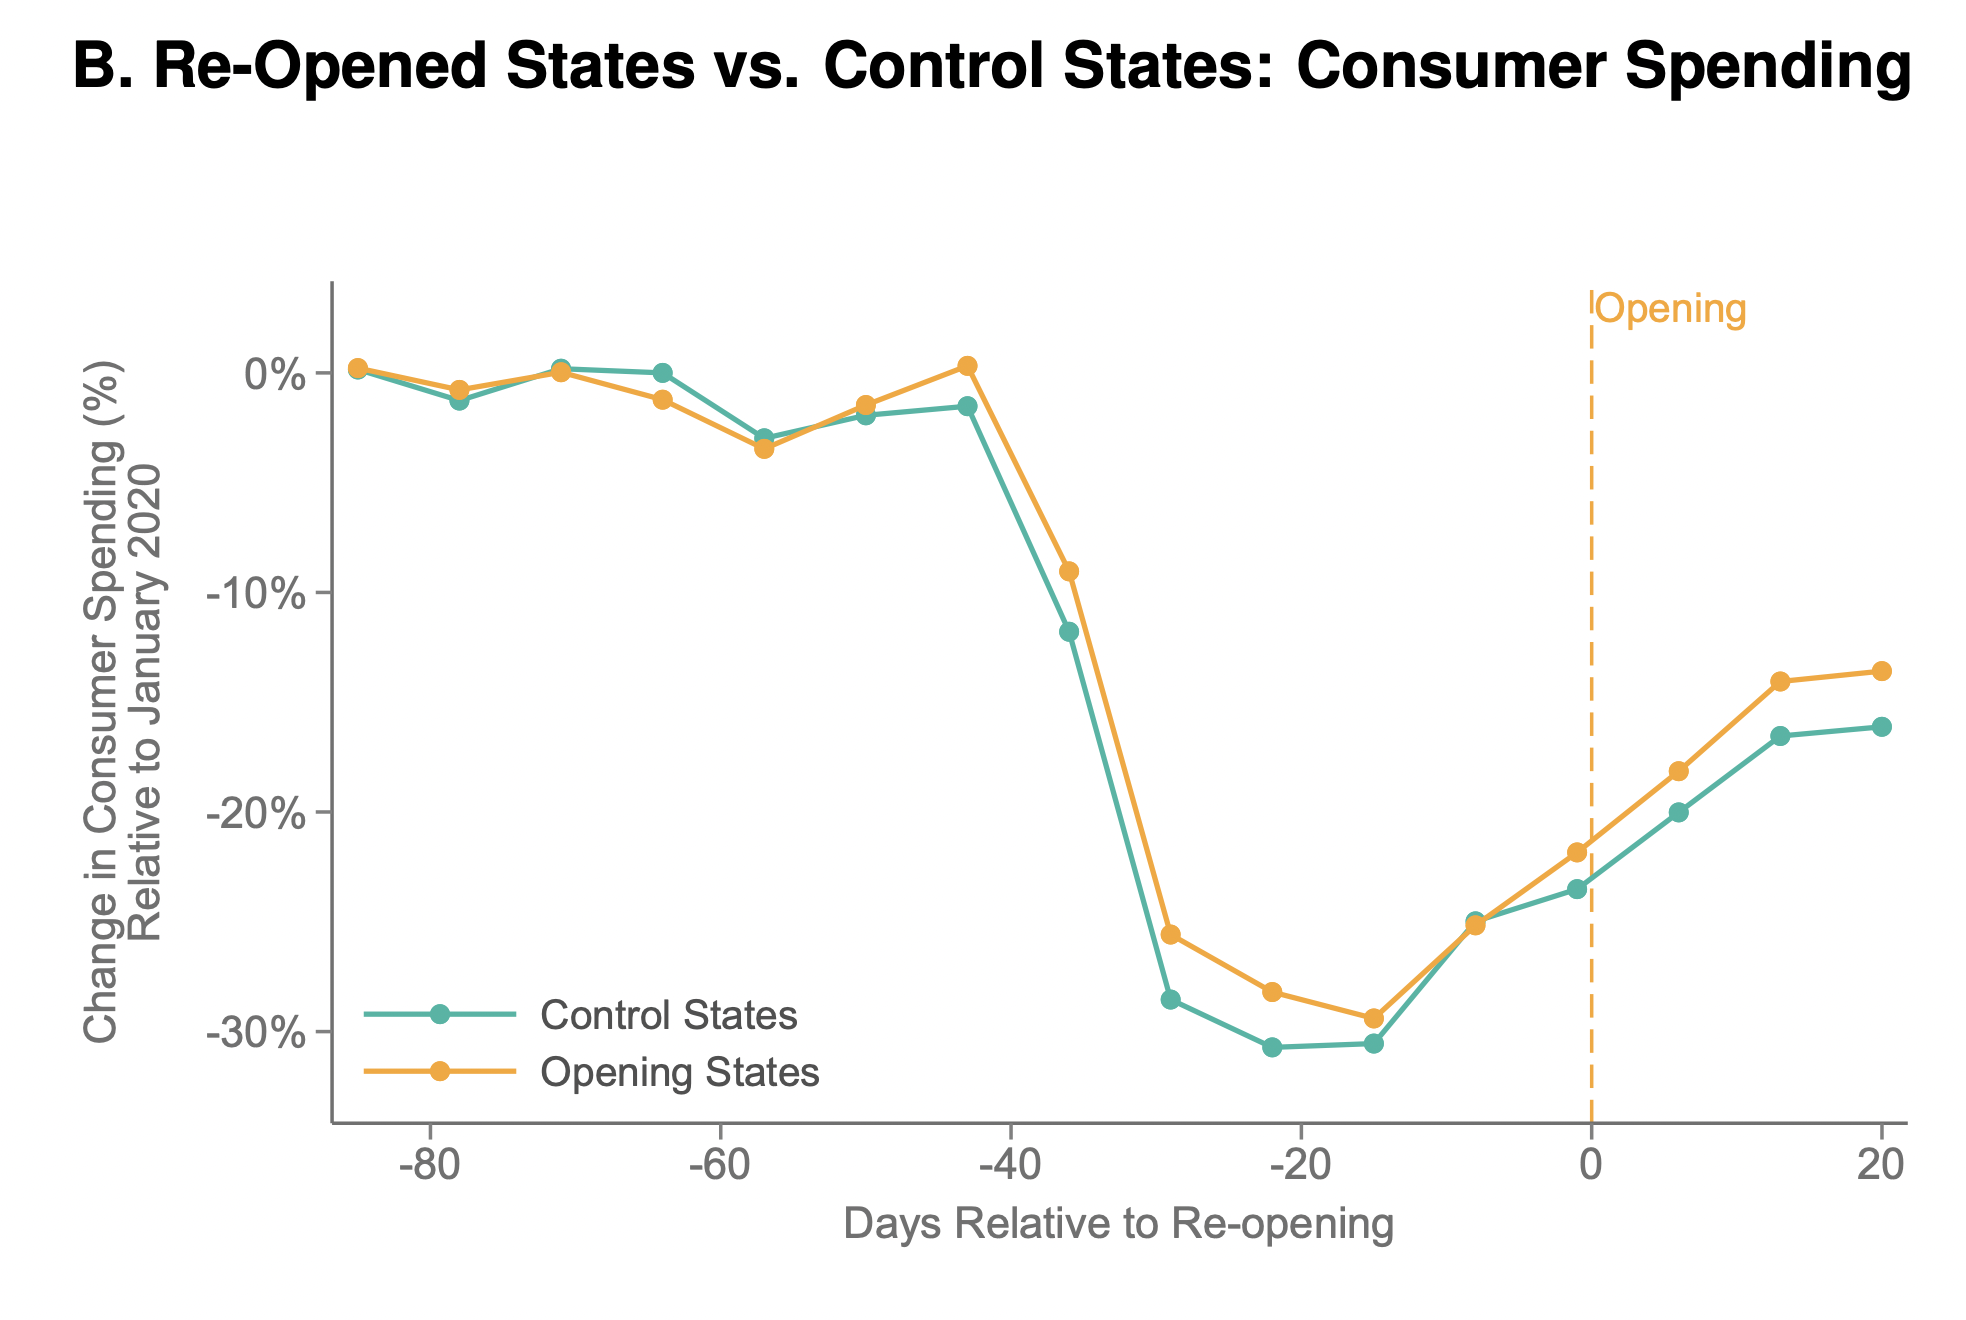
\includegraphics[width=\linewidth]{ChettySpendingGraph.png} 
        \caption{Chetty (2020)} 
        \label{fig:spendC}
    \end{subfigure}

    \begin{subfigure}[t]{0.8\textwidth}
        \centering
        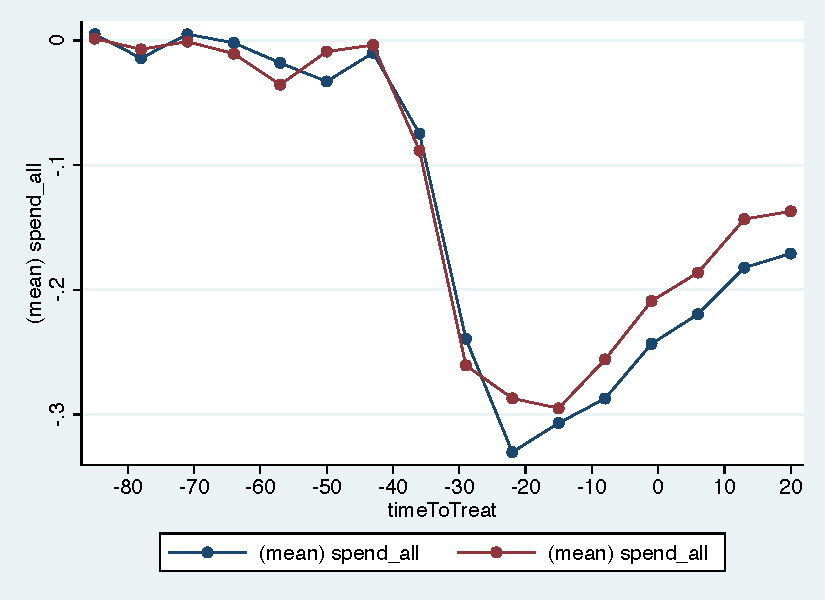
\includegraphics[width=\linewidth]{SpendingGraph.pdf} 
        \caption{Replication} 
        \label{fig:spend}
    \end{subfigure}
\end{figure}

\clearpage

\begin{figure}
    \centering
    \caption{}
    \begin{subfigure}[t]{0.8\textwidth}
        \centering
        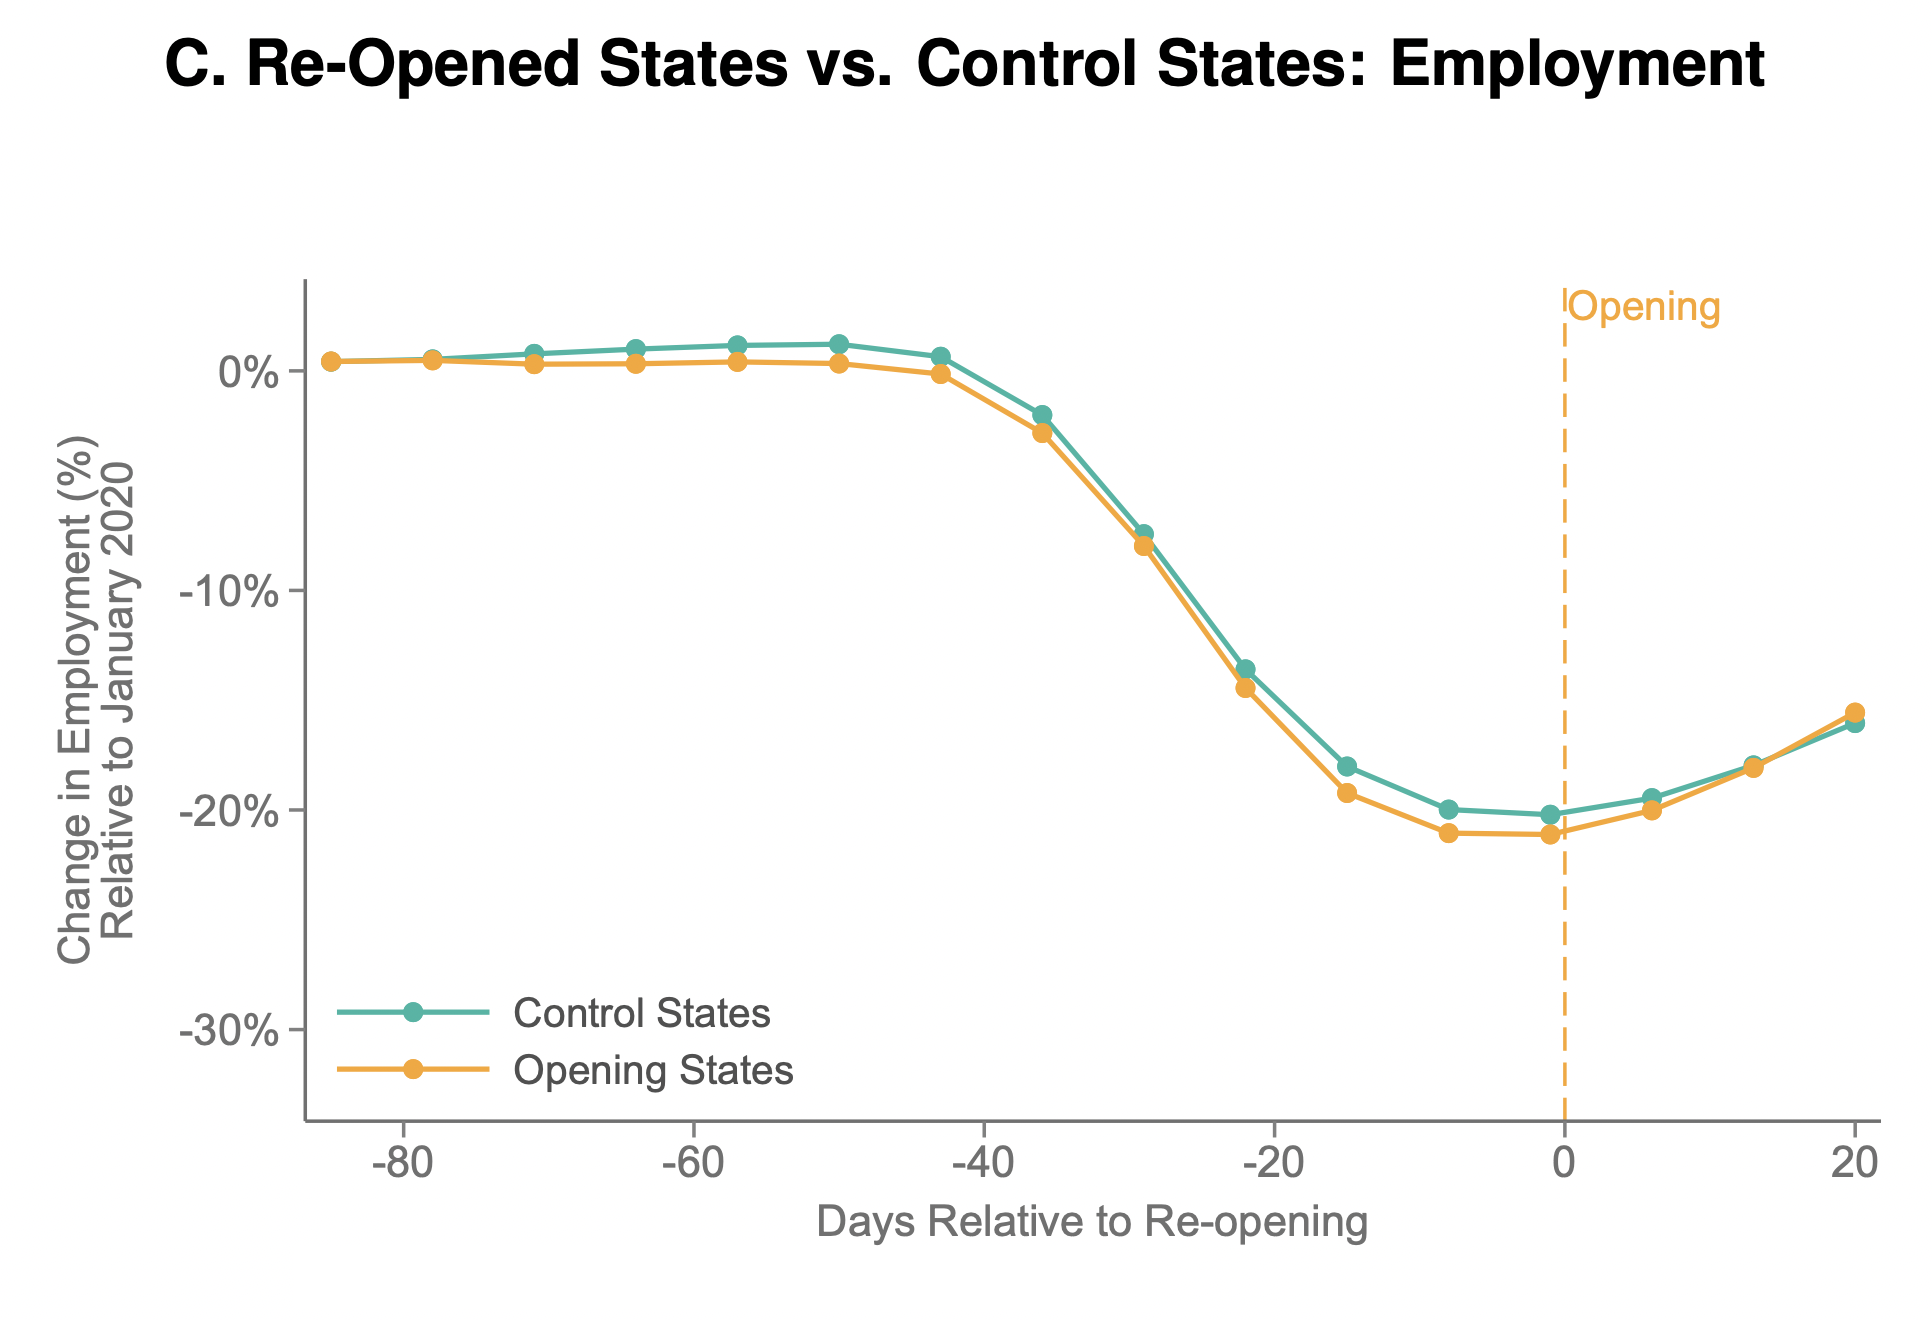
\includegraphics[width=\linewidth]{ChettyEmploymentGraph.png} 
        \caption{Chetty (2020)} 
        \label{fig:empC}
    \end{subfigure}

    \begin{subfigure}[t]{0.8\textwidth}
        \centering
        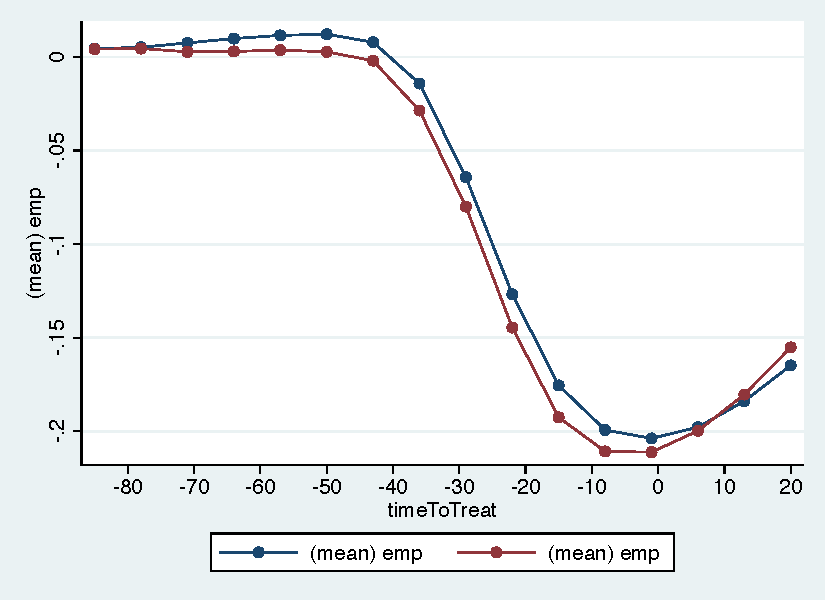
\includegraphics[width=\linewidth]{EmploymentGraph.pdf} 
        \caption{Replication} 
        \label{fig:emp}
    \end{subfigure}
\end{figure}

\clearpage

\begin{figure}
    \centering
    \caption{}
    \begin{subfigure}[t]{0.8\textwidth}
        \centering
        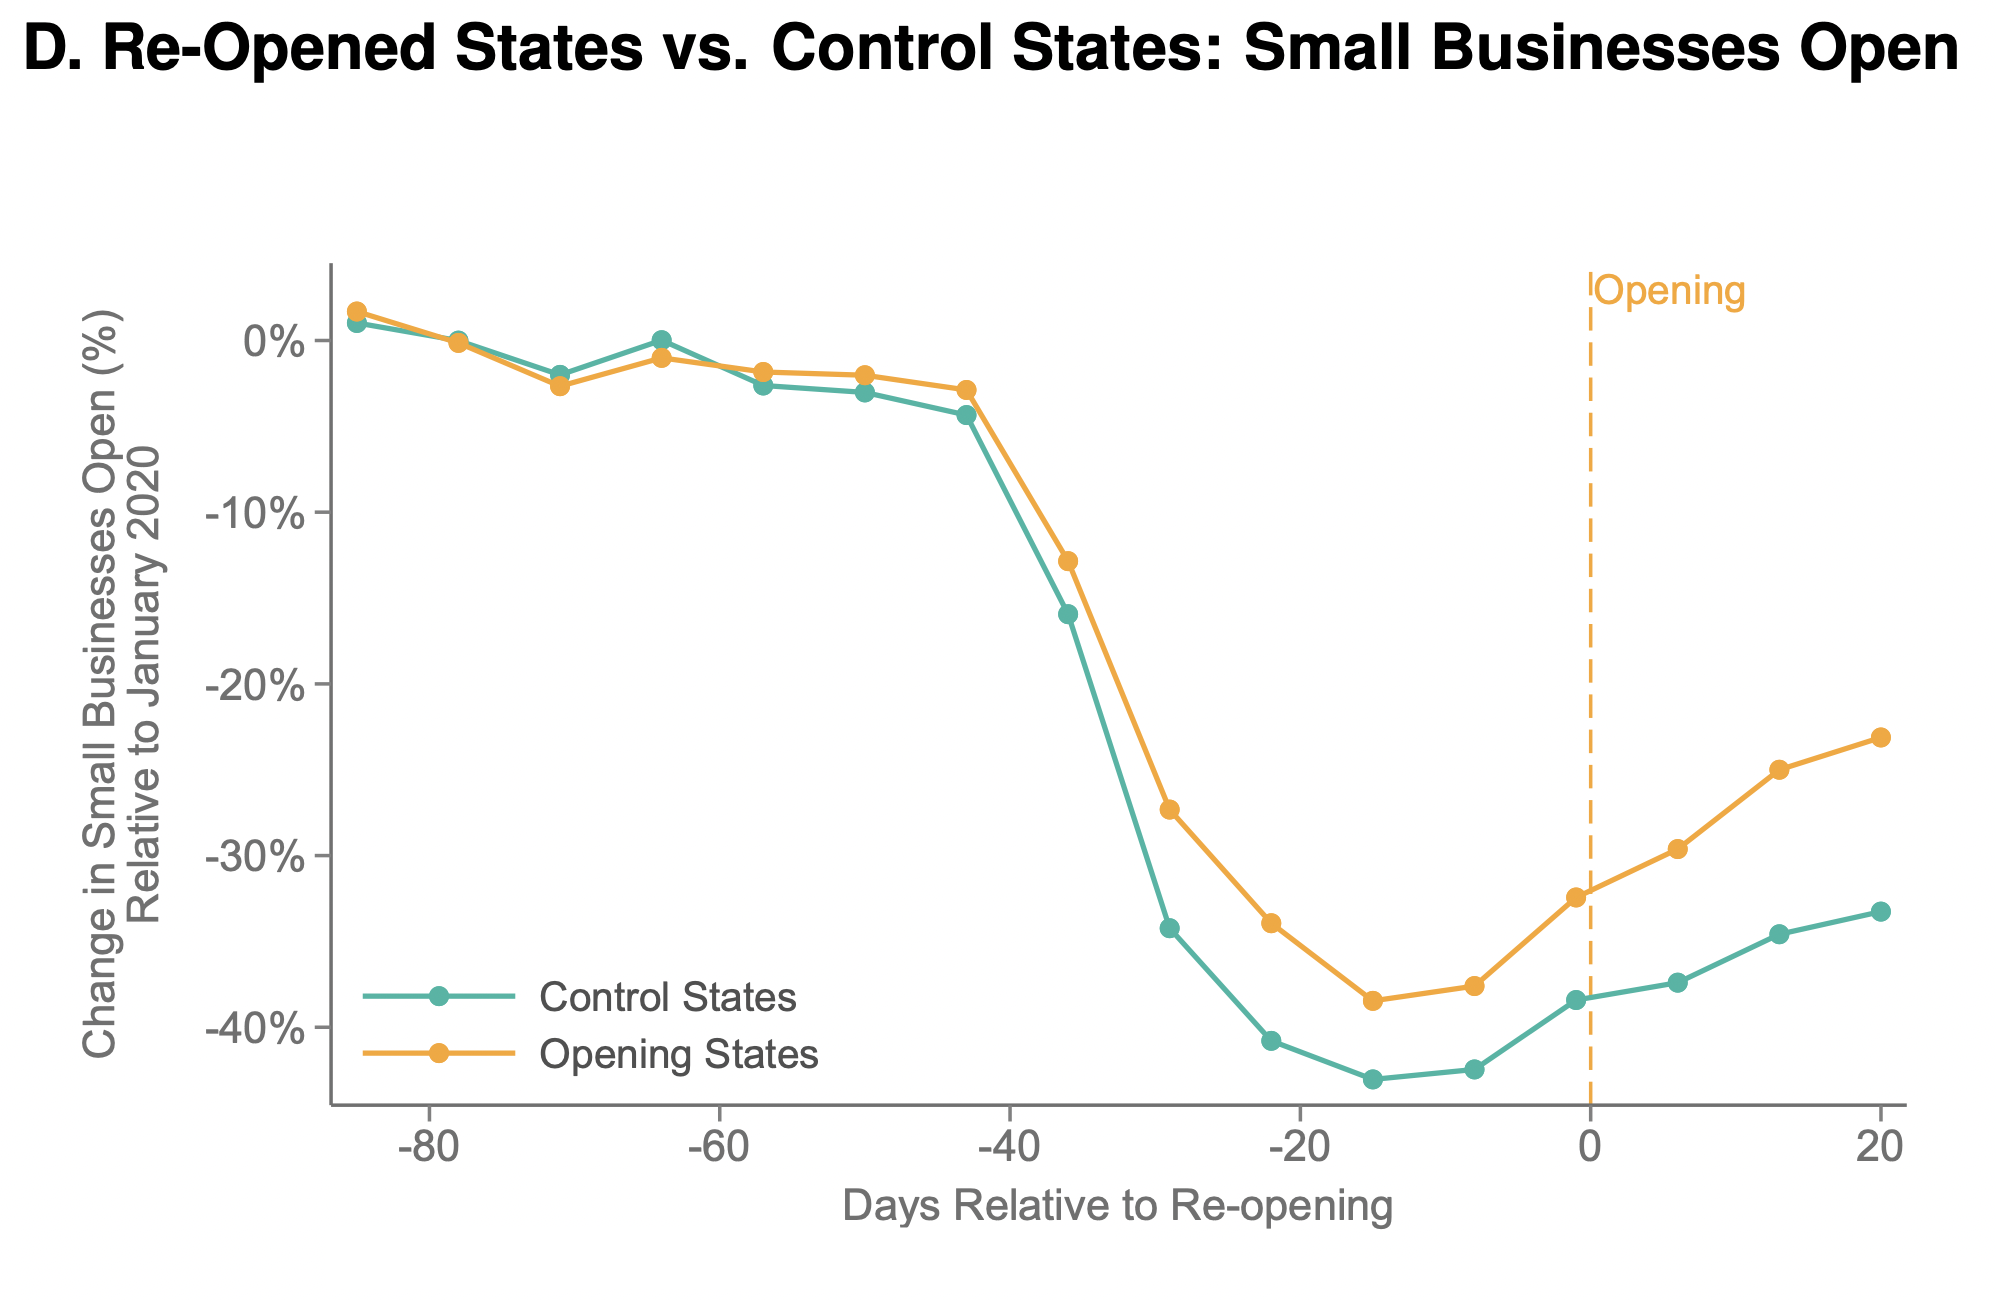
\includegraphics[width=\linewidth]{ChettySmallBusinessGraph.png} 
        \caption{Chetty (2020)} 
        \label{fig:merchantsC}
    \end{subfigure}

    \begin{subfigure}[t]{0.8\textwidth}
        \centering
        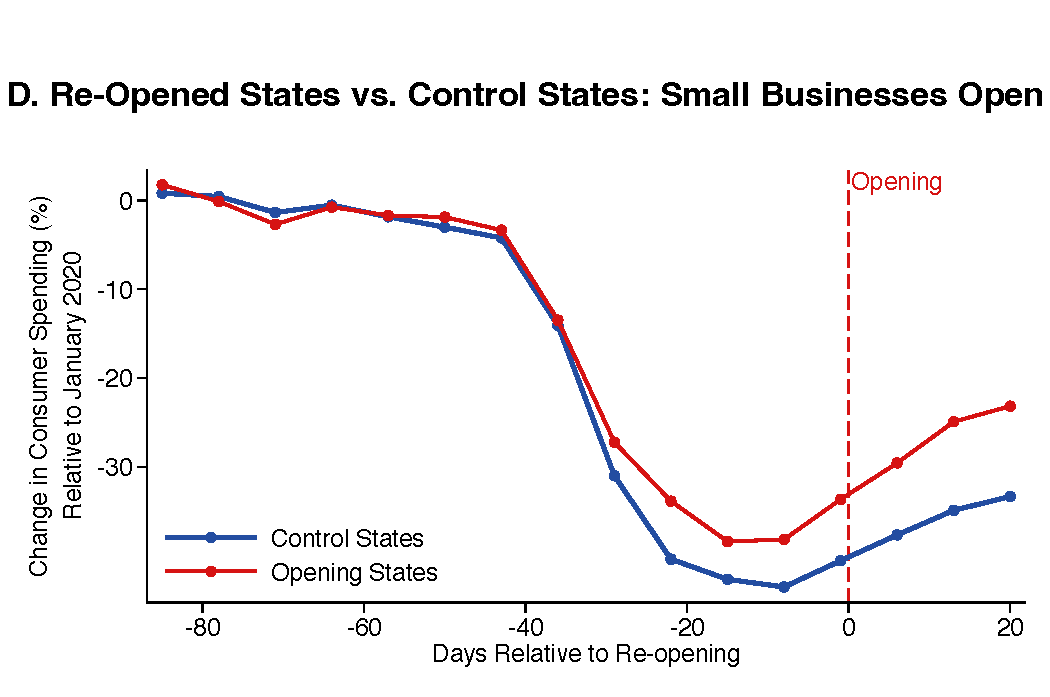
\includegraphics[width=\linewidth]{SmallBusinessGraph.pdf} 
        \caption{Replication} 
        \label{fig:merchants}
    \end{subfigure}
\end{figure}

\end{document}
